\begin{figure}[ht]
% \small
\centering
\captionof{table}{Main AUROC results. AUROC and Q\&A values are percentages, averaged over ten data points (five datasets and two phrasings). The $p < 10^{-4}$ columns indicate how many of those ten data points yielded $p$-values below $10^{-4}$ for the null hypothesis that AUROC $= 50\%$. The $p$-values are from the Mann-Whitney \emph{U} test; see Section~\ref{sec:method} for details.}
\label{tab:auroc}
\vspace{-.05 in}
\begin{tabular}{l c c c c c}
\toprule
& & \multicolumn{2}{c}{MSP} & \multicolumn{2}{c}{Max Logit} \\ 
LLM & Q\&A accuracy & AUROC & $p < 10^{-4}$ & AUROC & $p < 10^{-4}$ \\ 
\cmidrule(lr){1-1} \cmidrule(lr){2-2} \cmidrule(lr){3-4} \cmidrule(lr){5-6} 
Falcon 7B & 30.1 & 52.0 & 1/10 & 51.9 & 1/10\\
Falcon 40B & 40.5 & 60.2 & 7/10 & 58.6 & 7/10\\
Llama 2 7B & 39.7 & 58.6 & 6/10 & 57.8 & 7/10\\
Llama 2 70B & 58.7 & 71.1 & 10/10 & 66.9 & 9/10\\
Llama 3.0 8B & 59.1 & 71.2 & 10/10 & 68.9 & 10/10\\
Llama 3.0 70B & 78.8 & 81.3 & 10/10 & 68.4 & 9/10\\
Llama 3.1 8B & 62.0 & 72.9 & 10/10 & 67.3 & 10/10\\
Llama 3.1 70B & 80.6 & 83.4 & 10/10 & 69.6 & 10/10\\
Mistral 7B & 57.0 & 66.1 & 10/10 & 62.8 & 10/10\\
Mixtral 8x7B & 69.9 & 70.0 & 10/10 & 60.5 & 8/10\\
SOLAR 10.7B & 67.5 & 71.8 & 10/10 & 66.8 & 10/10\\
Yi 6B & 49.6 & 67.0 & 10/10 & 60.4 & 10/10\\
Yi 34B & 69.1 & 75.8 & 10/10 & 69.0 & 10/10\\
GPT-3.5 Turbo & 67.5 & 76.1 & 10/10 & -- & --\\
GPT-4o & 86.9 & 85.3 & 10/10 & -- & --\\
\bottomrule
\end{tabular}

\vspace{.6 in}
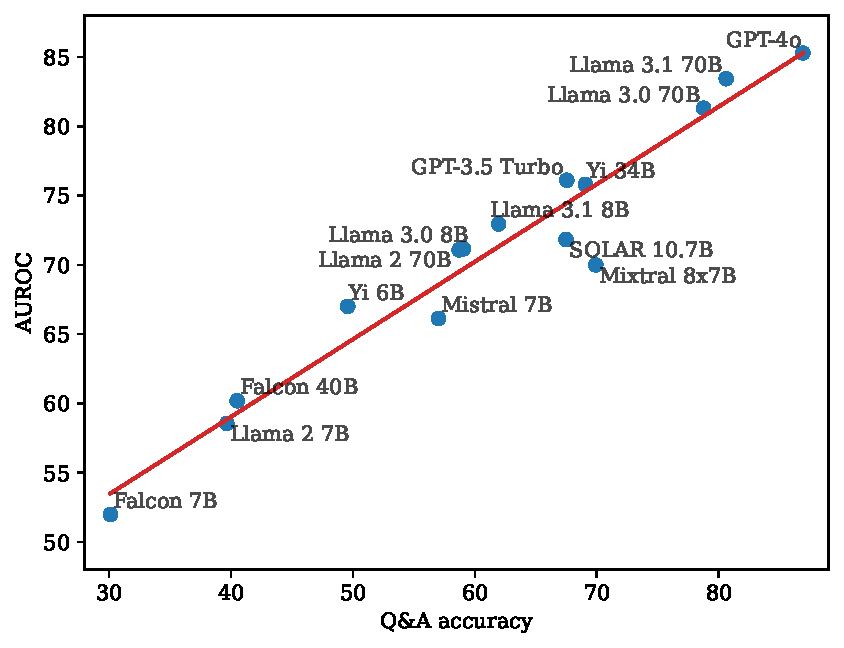
\includegraphics[scale=\figscalelarge]{figs/chat_figs/acc_vs_auc_prob_max_r2_0.942_p_0.00000.pdf}
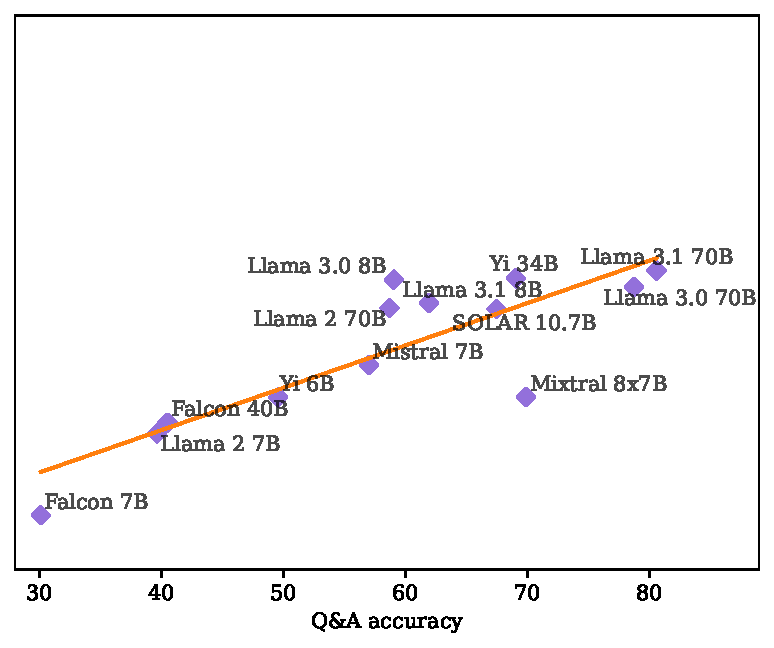
\includegraphics[scale=\figscalelarge]{figs/chat_figs/acc_vs_auc_logit_max_r2_0.714_p_0.00028.pdf}
 % \vspace{-.1 in}
\captionof{figure}{Average AUROC vs average Q\&A accuracy for the MSP (left) and Max Logit (right). These plots use the same data as Table~\ref{tab:auroc}. The coefficients of determination for MSP and Max Logit were $R^2=0.94$ and $R^2=0.71$ respectively, both with $p <10^{-3}$, indicating strong correlations.}
\label{fig:auroc-qa}
 % \vspace{-.1 in}
\end{figure}


